\vspace{-0.4cm}
\section{Introduction}

Navigation systems have changed the way we drive and in particular affected how
we plan our trips. Nowadays, they are not only used to find the fastest
route in an unknown area but also to react to current events such traffic jams
and accidents on an everyday route. The latter became possible due to the
availability of real-time traffic data, amongst others, from road sensors, GPS
transmissions from vehicles and reporting tools for accidents. The most recent
navigation systems (e.g., \cite{PanDemShaGup13}) even go one step further and
use the collected historic data to build traffic models in order to predict the future traffic. In
conjunction with the real-time information the ultimate goal is to provide a faster
route and better estimation of the expected travel time to the user. A
main observation to be made here is that, since in these systems a prediction
component is involved, the outcome (i.e., the estimated time for a route and
thus the fastest route) can never be trusted with certainty but is
obviously subject to variation. Following this thought the fastest route is not
necessarily the most reliable route, i.e., the route with the least variation in
possible travel times. Reliability of a route is particularly important to users
when a deadline, such as a flight departure or an important meeting, has to be
met. 

% Shortest path problem in directed weighted graph is one of the most fundamental
% optimization problems. The most popular and widely used application of shortest
% path problem is to find the fastest route on road networks, which are modeled as
% graph and travel times are applied as weight on the edges. 
% 
% In reality, the travel-time (weight) to traverse a street (edge) of the road
% network (graph) is subject to variations such as traffic jams, weather
% conditions, accidents and much more. The key factor to compute the fastest path
% on road networks is thus the accuracy of the travel times on the edges. Recent
% advances in sensor networks and location based services have enabled collecting
% traffic data from roadside sensors and smartphones, and hence it is now
% feasible to accurately capture the travel-time on the edges (link travel time)
% in real-time.
% 
% Recent studies (e.g.,\cite{DemiryurekSSD11,PanDS12}) suggest that relying on the current link travel time is still not sufficient for an accurate computation of the shortest path.
% The main problem is that the link travel times obviously keep changing
% while the user who issued the query is traveling. To cope with this issue
% algorithms for time-varying traffic networks have been proposed. In practice the application of these algorithms is
% complicated by the fact that the future travel times of edges are not known by
% the time the query is issued but have to be predicted. This prediction
% brings the notion of uncertainty to this problem. Now the time to traverse an
% edge does not only change while the vehicle of the user is in motion but is
% also uncertain. Obviously these considerations have an effect on the travel
% time for a route consisting of several edges. One possible way to deal with this
% uncertainty is to get rid of it and for example use the expected travel time
% for the edges or the whole route. However, recent studies have shown that this
% methodology gives away a wealth of information that can be
% utilized \cite{Sarma08}.

To illustrate, consider the example in Figure \ref{fig:motivation1}, where
estimated total travel times of two paths are given. Based on these expected
travel times (as returned by traditional approaches), route A is clearly
the one to be preferred. However, this result ignores uncertain nature of the
traffic prediction and only feigns certainty. Let us now consider Figure \ref{fig:motivation2}, where the travel times for
both routes are taking the uncertainty of the prediction into account, i.e., the
travel times are given by a probability density function (\textit{pdf}).
Continuing with our example in Figure \ref{fig:motivation}, let's assume that the user has only 60  minutes to reach
the destination in order to be on time. The probability that the user is at the
destination in at most 60 minutes, is the sum of probabilities for times
smaller or equal to 60 minutes. Under this consideration the user has a
probability of 89\% of reaching his destination in time when choosing route A
(implying that he will be late in one out of nine times), and a 99.2\%
probability when choosing route B. Furthermore, if the user wants to achieve the
same level of confidence using route A, he has to start 10 minutes earlier.

% \begin{figure}[h]
%     \centering
%     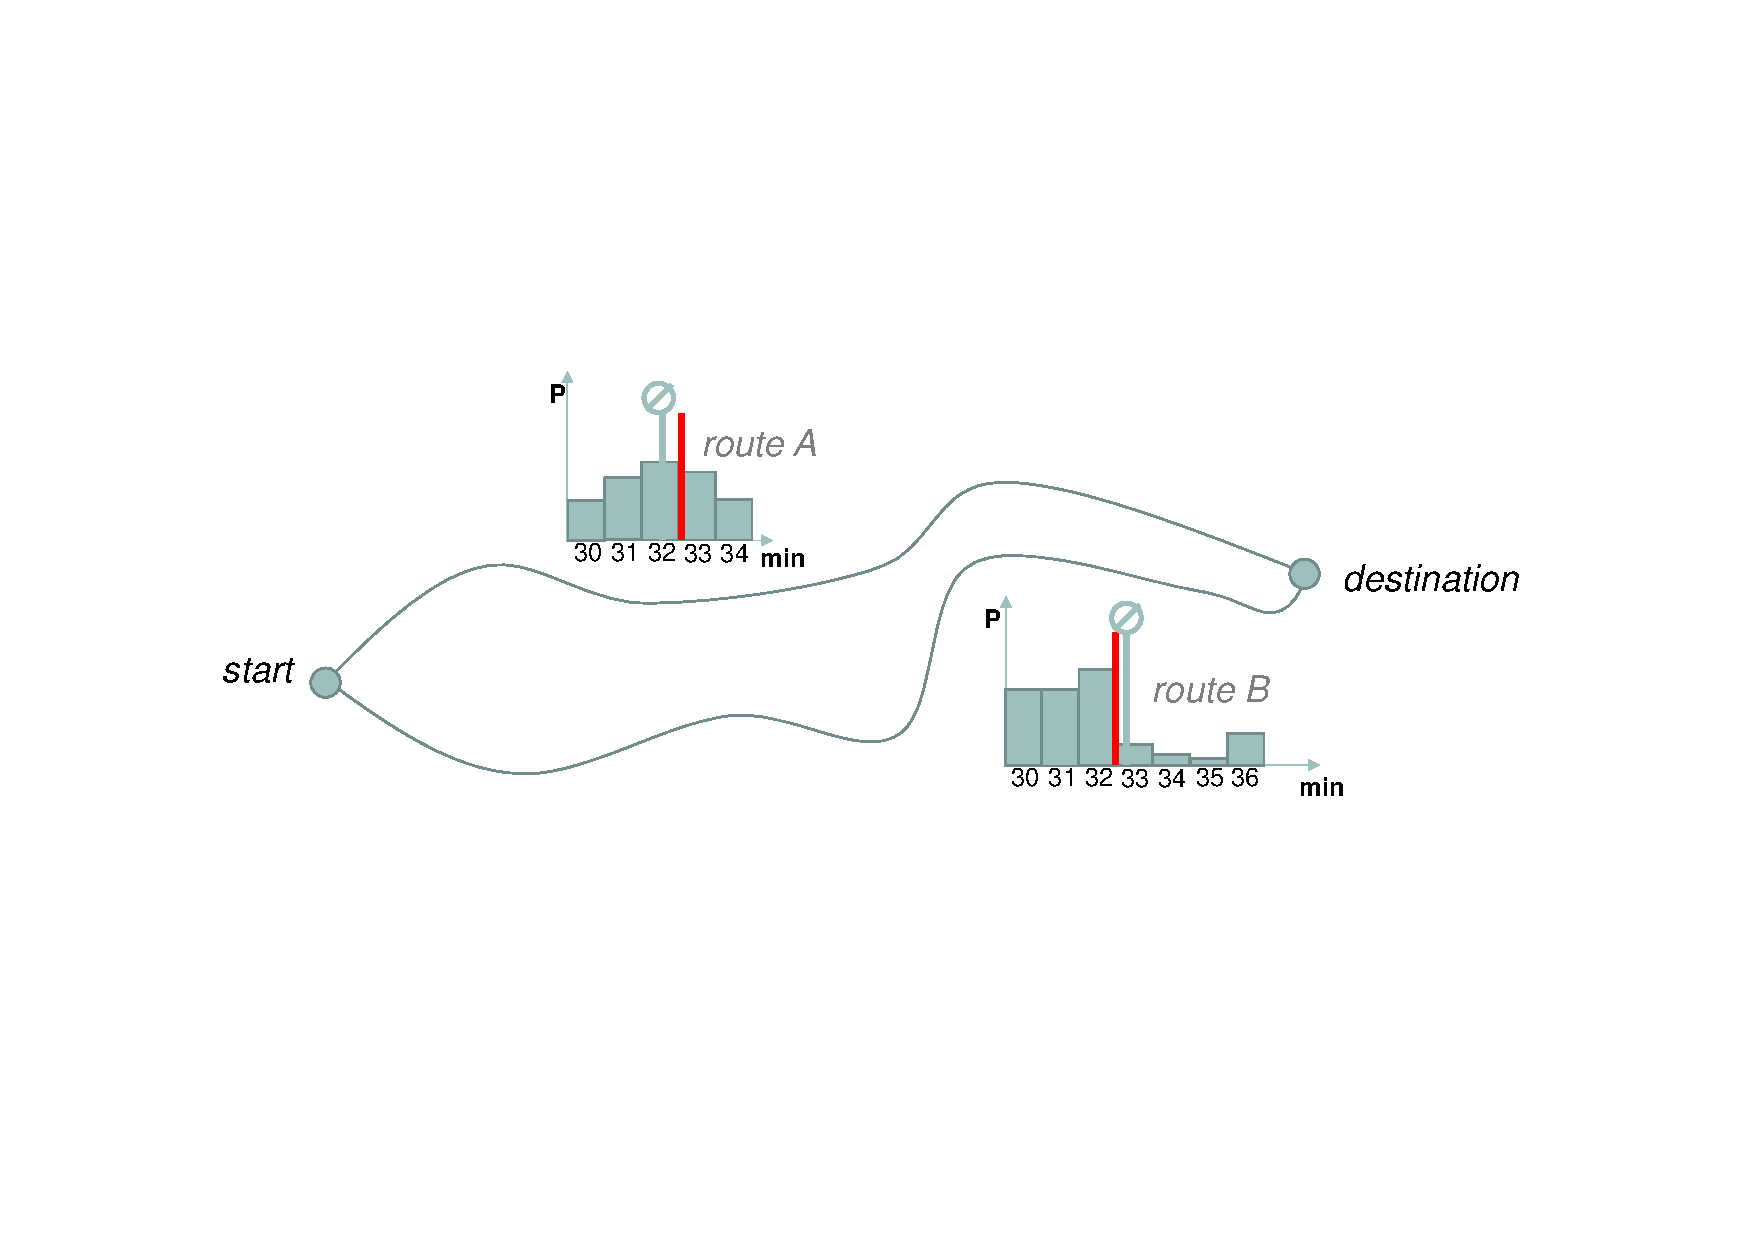
\includegraphics[width=0.90\columnwidth]{figures/motivation.pdf}
%     \caption{Probabilistic cost of two routes}
%     \label{fig:motivation}
% \end{figure}

\begin{figure}[t]
    \centering
    \subfigure[Deterministic result]{
        \label{fig:motivation1}
        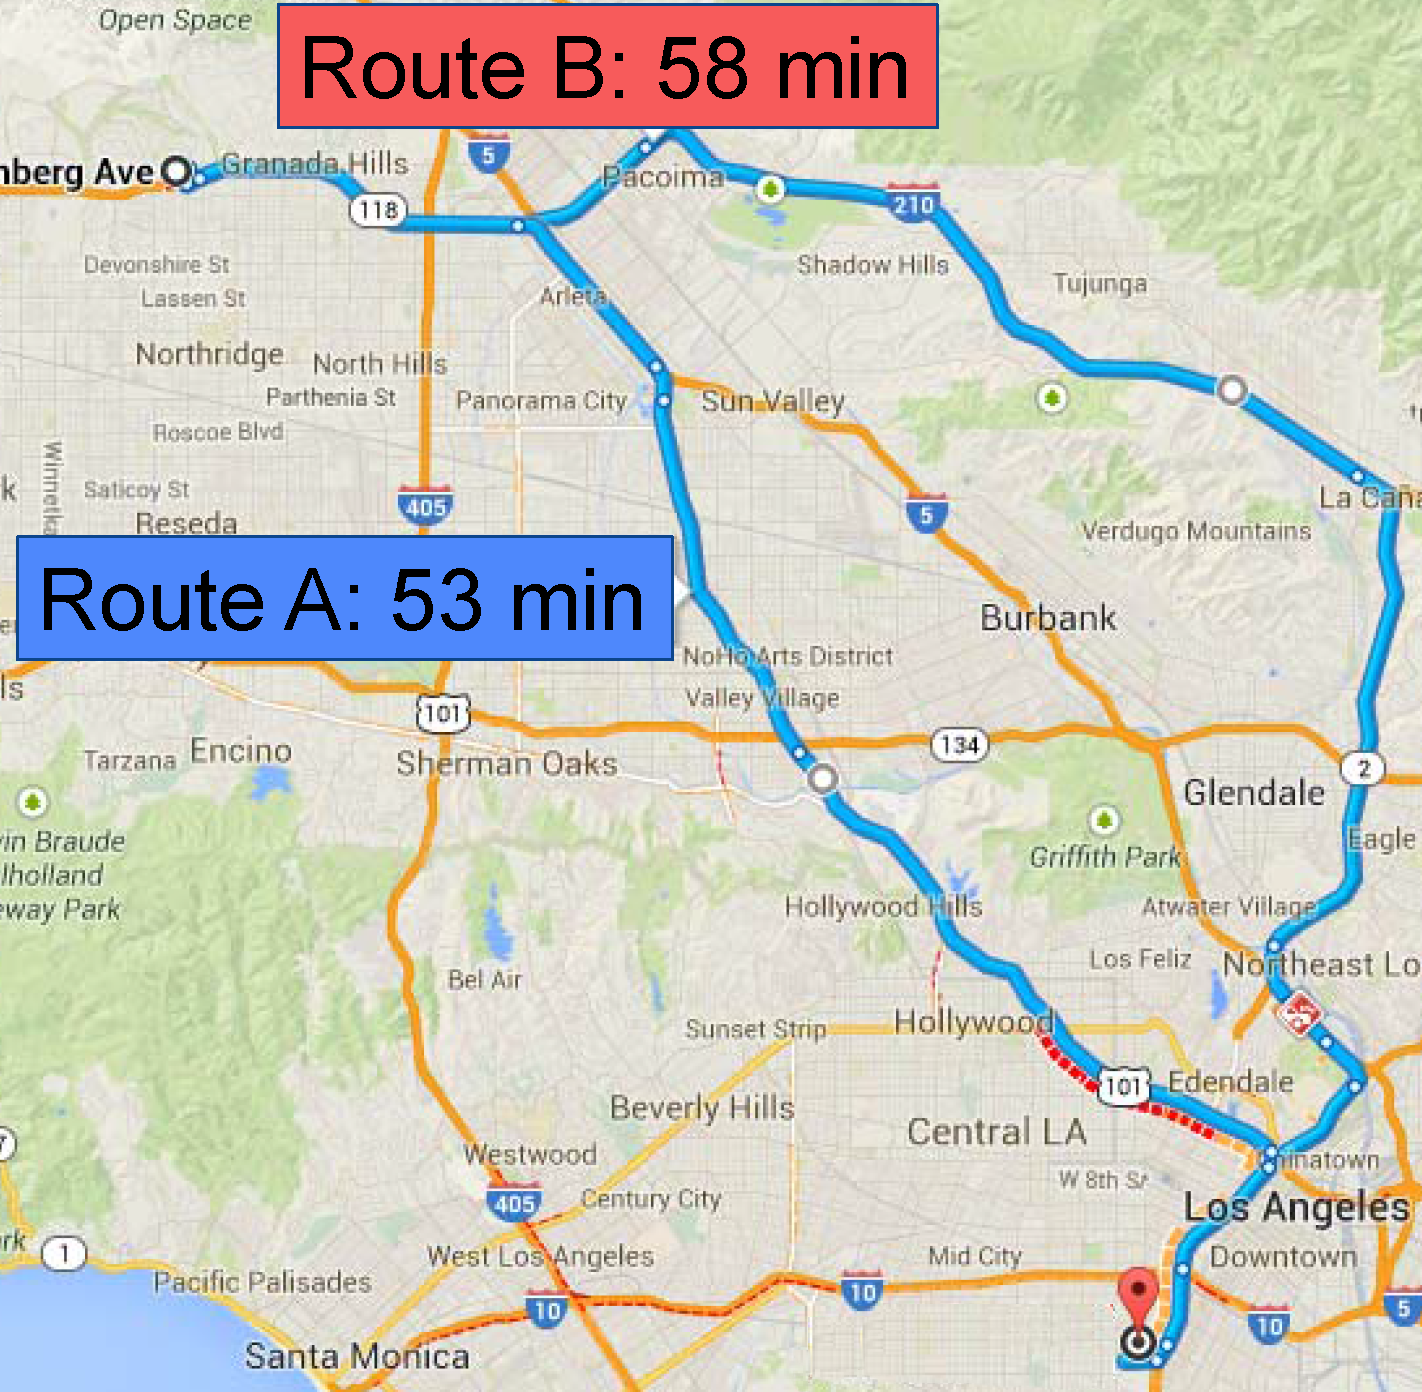
\includegraphics[width =
        0.38\columnwidth]{figures/motivation1_anonym.png} }
    \subfigure[Probabilistic result]{
        \label{fig:motivation2}
        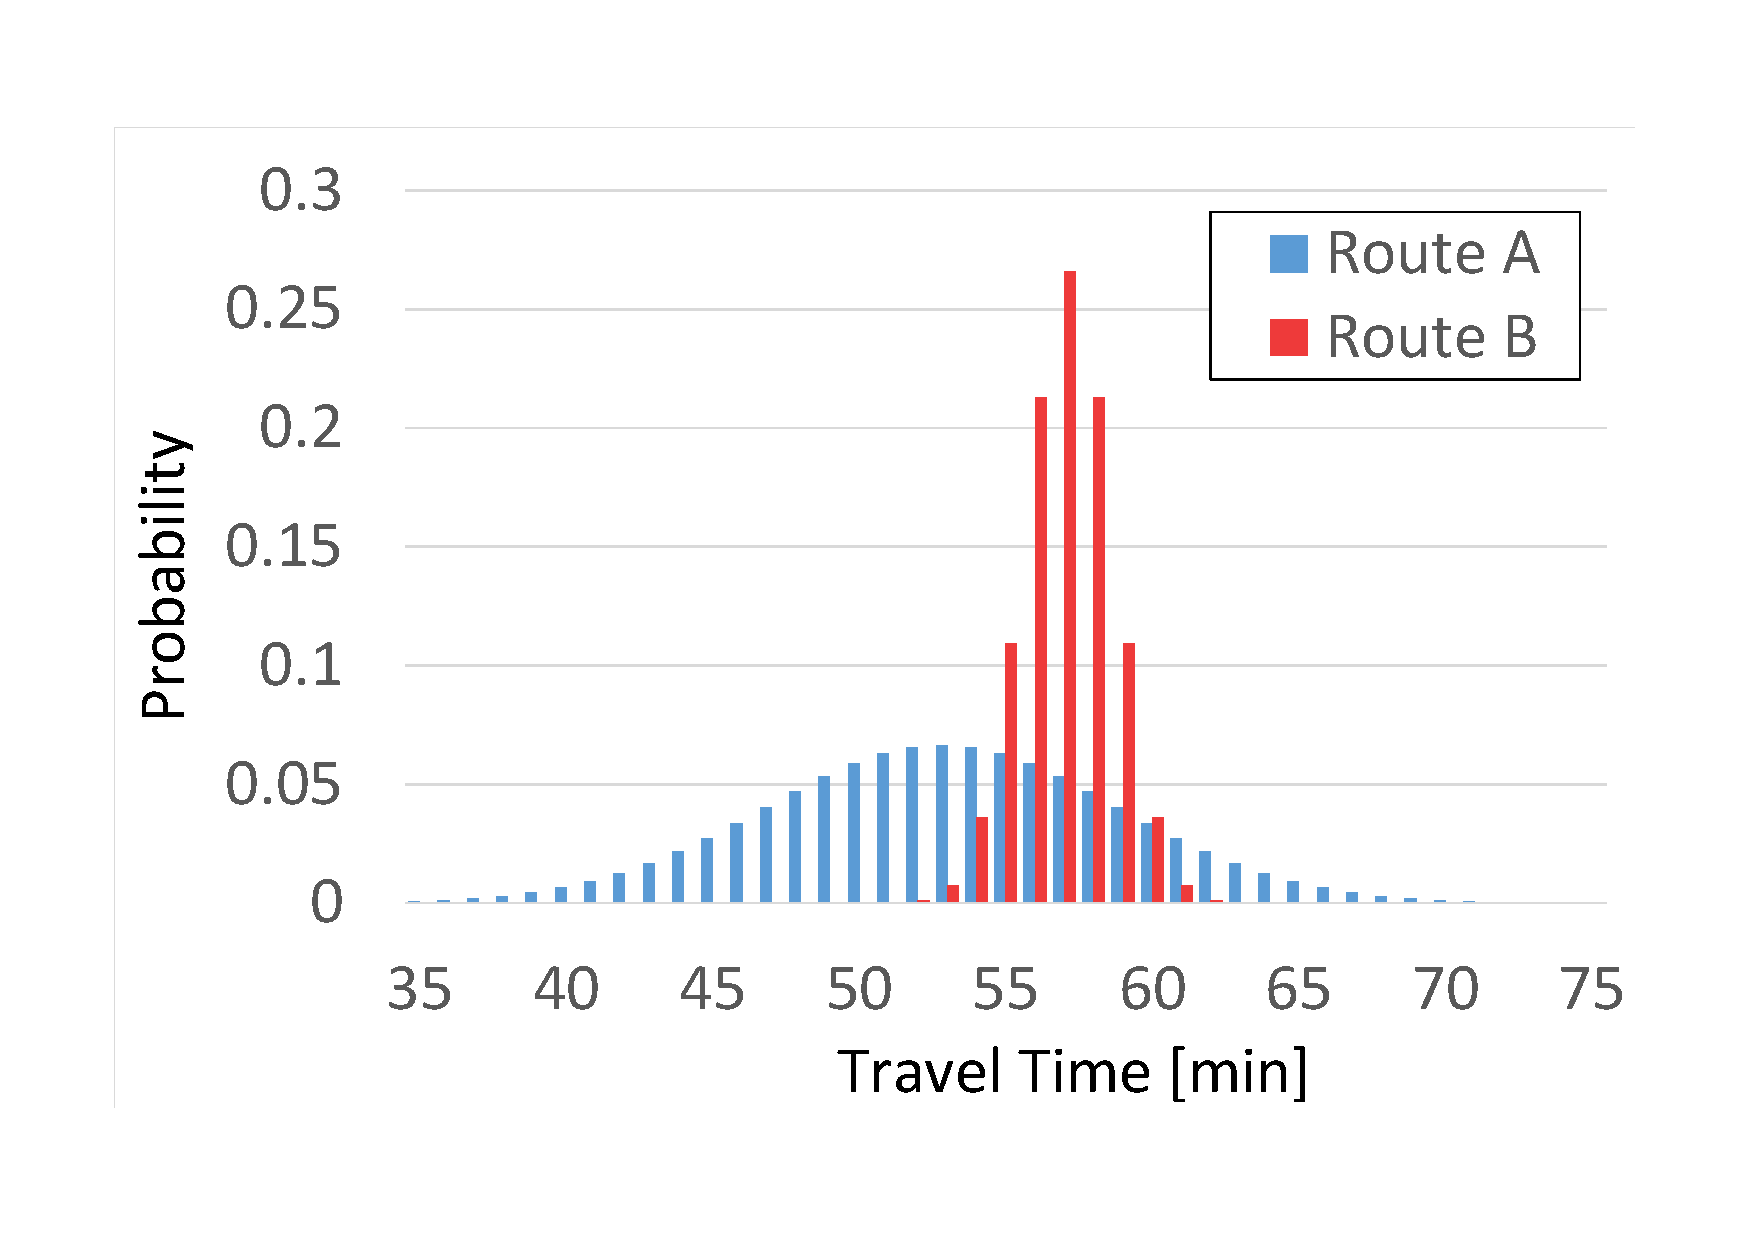
\includegraphics[width = 0.53\columnwidth]{figures/motivation2.pdf}
    }
    \vspace{-0.2cm}
    \caption{Estimated Travel Time of two paths}\label{fig:motivation}
    \vspace{-0.5cm}
\end{figure}

The above example shows that similar to other applications
\cite{Sarma08}, explicitly handling the uncertainty is better than ignoring it.
Correspondingly, we believe that taking the uncertainty of the travel time into account will
enable next-generation route planning applications by extending path queries to
probabilistic path queries, allowing for queries such as:  \textit{What are the
paths from my hotel to the airport whose travel time is at most 40 minutes with a probability of at least
95\%?}. 

% Recently, some studies have considered variations of the shortest-path
% problem under consideration of uncertainty (cf Section \ref{sec:related}) in
% the travel time. These studies reveal a plethora of useful scenarios and queries
% which can be enriched by confidence when taking this uncertainty into account.

With this goal in mind, in this work, we consider the problem of
computing the \textit{pdf} of the travel time for one given path. This
\textit{pdf} associates each possible travel time with the corresponding
probability that the vehicle will need this time for completing the route.
Specifically, we will make the following contributions:

\begin{enumerate}
  \item \label{item:1} It turns out that all existing approaches considering uncertainty in traffic
networks make the simplifying assumption that the probabilistic link travel
times (\textit{pltts}), i.e., the predicted time for each road segment, are
given. However, existing techniques on predicting link travel times provide a
single value estimation only or are not compatible with existing techniques for
computing the probabilistic link travel time of a path. Thus, there is a huge
lack in taking the uncertainty of predictions into account and estimating not
only accurate \textit{pltt} estimations but also possible correlations between them. We
will fill this gap by providing techniques that yield \textit{pltts} by taking historic
as well as real-time information into account.
  \item \label{item:2} Subsequently we focus on approaches for computing the
  probabilistic path travel times based on \textit{pltts}. After reviewing and categorizing the existing studies
 considering uncertainty in networks, we identify three basic characteristics
 (representation, time-dependency and correlation) and extract or adapt
 methods for all possible combinations of these characteristics for the ultimate
 goal of a fair and insightful comparison.
  \item The evaluation  of a probabilistic prediction is a daunting task.
  Neither expected distance measures nor goodness-of-fit methods nor primitive scoring
  functions are applicable. So far no evaluation of the accuracy for the
  methods in item \ref{item:2} has been performed. We propose adequate solutions to the evaluation problem and compare
  the accuracy of both the techniques in items \ref{item:1} and \ref{item:2} on
  a large real-world data set. Our results provide deep insights on the effect
  and functionality of all sub-modules.
\end{enumerate}

For the ultimate goal of providing this pipeline we avail ourselves of
techniques from database, transportation, weather prediction and statistics
research. One main question that this study will thus address is the
usefulness and validity of the consideration of uncertainty for route 
planning applications.
% 
% \begin{itemize}
%   \item We review and categorize existing work for shortest path algorithms on
%   uncertain traffic networks with a particular focus on the computation of the
%   uncertain travel time of one path.
%   \item We consider the problem of the parameter generation. This involves
%   estimating uncertain link travel times and correlations between these.
%   \item 
%   \item All experiments are carried out on a large scale real-world dataset
% \end{itemize}

% The remainder of this paper is structured as follows: In Section
% \ref{sec:problemdef} we formally define the problem setting and crucial notations. We review
% important related work in Section \ref{sec:related}. In Section
% \ref{sec:lttestimation} we propose methods for the probabilistic prediction of
% edge weights and correlations. How these predictions can be used in order to
% compute a prediction for a whole path is discussed in Section \ref{sec:methods}.
% We then discuss measurements for evaluating probabilistic predictions in Section
% \ref{sec:evaluate}. In a broad experimental setting we show both the validity of
% the proposed estimation methods for the link travel times and a comparison of
% the approaches in terms of efficiency and accuracy in Section
% \ref{sec:experiments}. Section \ref{sec:conclusion} concludes the paper.

% Figure \ref{fig:component} illustrates the components of this work.
% \begin{figure}[h]
%     \centering
%     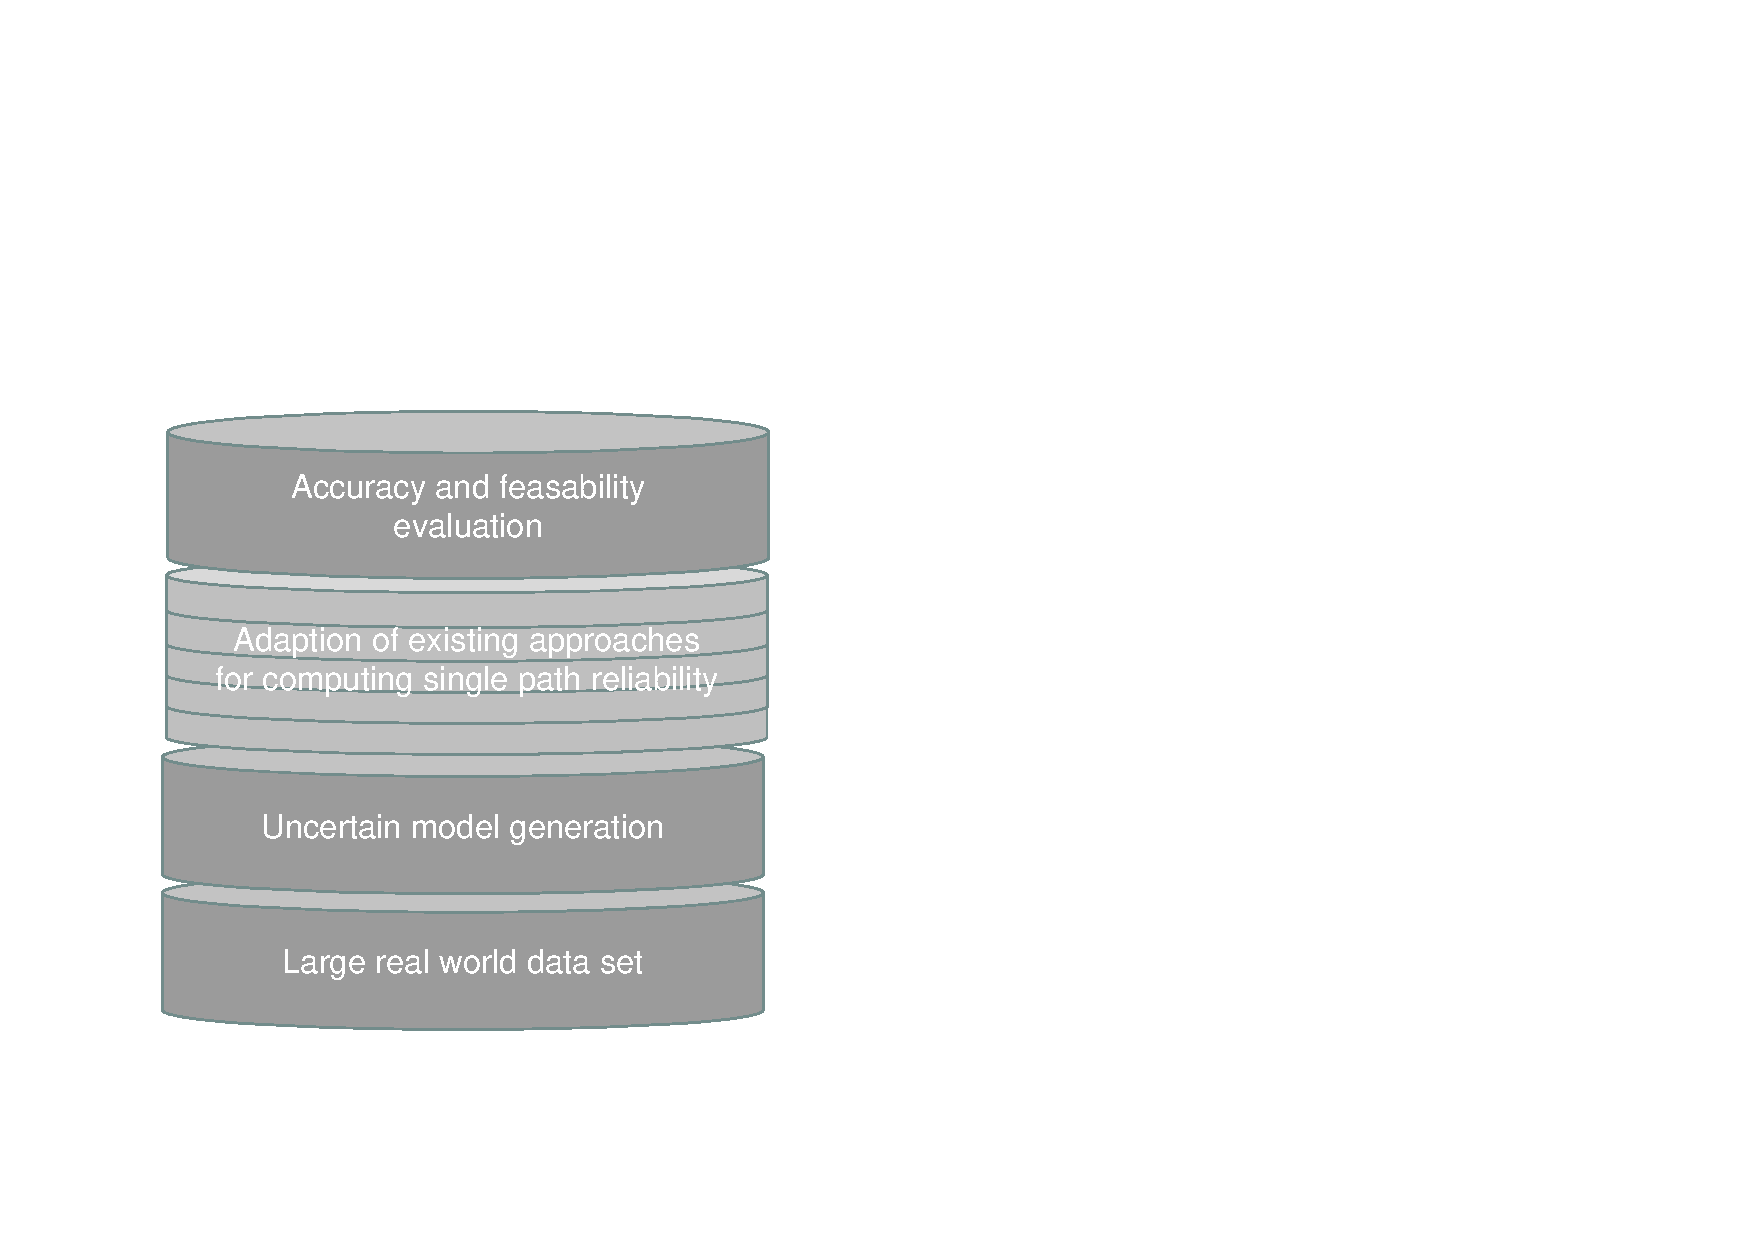
\includegraphics[width=0.50\columnwidth]{figures/contributions.pdf}
%     \caption{Components of this work}
%     \label{fig:component}
% \end{figure}


% ------Copy from \cite{NieWu09}-----------
% Another common definition of optimality in stochastic routing has to do with reliability, recognizing that a LET route (or
% policy) may be subject to high risks and therefore is not desirable to a
% risk averse
% traveler. For example, people tend to budget
% a large amount of time for travel when they plan for important events (e.g. job interviews). The key objective of routing in
% such a circumstance is to reduce the risk of arriving late rather than to minimize the expected travel time. In practice, how-
% ever, such risk averse behavior leads to excessively conservative time budgets. It is therefore necessary to both guarantee
% reliable on-time arrival and avoid unnecessary waiting. This paper precisely addresses the above problem.
% ------Copy end -----------